% !TEX root = Bachelorarbeit Synthetische Daten.tex
\chapter{Methodisches Vorgehen} \label{ch:methodology}

In diesem Kapitel wird das methodische Vorgehen der Arbeit beschrieben. Als Basis für die Untersuchung der Forschungsfragen wird zunächst der MVIP-Datensatz vorgestellt, auf dem die Experimente durchgeführt werden. Anschließend wird die Implementierung der Modelle DA-Fusion und Supervised Contrastive Learning erläutert. Schließlich wird der Versuchsaufbau für die Generierung der synthetischer Daten mit DA-Fusion und die Trainings- und Testdurchläufe mit Supervised Contrastive Learning beschrieben.

\section{MVIP-Datensatz} \label{sec:dataset}

Grundlage der Forschungsarbeit ist der im Rahmen des EIBA-Projekts entstandene MVIP-Datensatz \parencite{Koch2023mvip}, wobei MVIP für \textit{Multi-View Industrial Parts} steht. Er enthält 308 Klassen, welche wiederum in 18 verschiedene Oberklassen (Super Classes) eingeteilt sind. Insgesamt gibt es etwa 71.276 Sets an Bildern, die jeweils RGB- und Tiefendaten, sowie Segmentierungsmasken enthalten. Die Bilddaten stammen aus Intel RealSense D435 und D415 Tiefenkameras, die die Objekte gleichzeitig aus verschiedenen Perspektiven aufnehmen.

Darüber hinaus gibt es auch Metadaten, etwa zum Gewicht des Objekts, oder Beschreibungen in natürlicher Sprache durch verschiedene Stichwörter (z.B. "Used", "Rusty", usw.).

\subsection{Teildatensatz} \label{subsec:subdataset}

% Wahl eines Teildatensatzes mit 20 "CarComponent" Klassen
Da relativ viele Trainings- und Testdurchläufe vorgesehen waren, war es notwendig, einen Teildatensatz auszuwählen, um die Rechenzeit zu reduzieren.

Konkret wurden 20 Klassen aus der Oberklasse "CarComponent" ausgewählt, da diese Objekte wie Motoren und Generatoren enthält, welche von den in \autoref{subsec:challenges-synt-data} beschriebenen Herausforderungen besonders betroffen sind. Insgesamt enthält der Teildatensatz 2390 Trainingsbilder und 1000 Validierungsbilder. Darüber hinaus kamen die Segmentierungsmasken in der Vorverarbeitung zum Einsatz, die im nachfolgenden Abschnitt behandelt wird. %In Anhang \ref{app:subdataset} sind die Klassen im Detail aufgeführt.

\begin{figure}[h]
	\centering
	%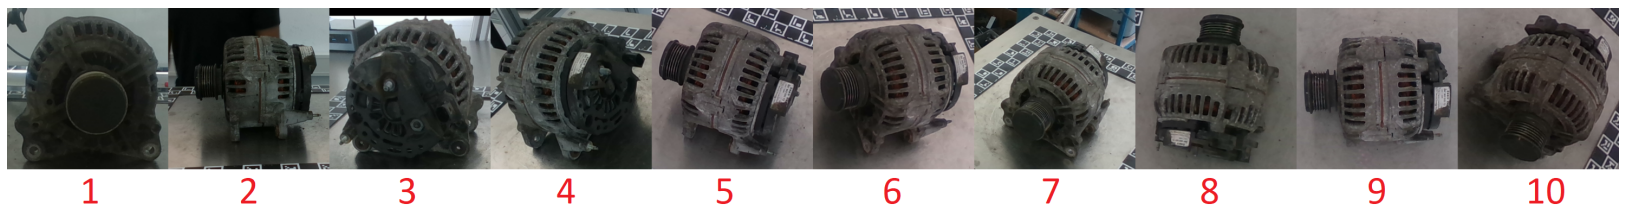
\includegraphics[width=\textwidth]{figure_mvip_ex_cropped_1.png}
	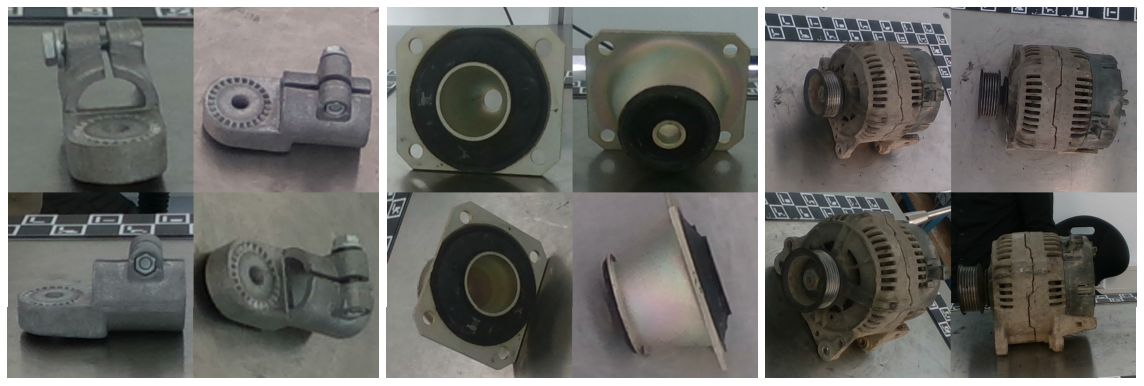
\includegraphics[width=\textwidth]{figure_mvip_ex_cropped_2.png}
	\caption[Beispielbilder aus dem MVIP-Datensatz, die auf die	Region of Interest (ROI) zugeschnitten wurden.]{Beispielbilder aus dem MVIP-Datensatz, die auf die\\
	Region of Interest (ROI) zugeschnitten wurden \parencite{Koch2023mvip}.}
	\label{fig:mvip-examples}
\end{figure}

\subsection{Vorverarbeitung} \label{subsec:preprocessing}

% ROI-Crop
Die Vorverarbeitung der Bilder unterscheidet sich nur leicht zwischen dem Fine-tuning der Text-Embeddings für DA-Fusion und den Trainings- und Testdurchläufen mit Supervised Contrastive Learning. In beiden Fällen wurden die Bilder auf die Region of Interest (ROI) zugeschnitten (siehe \autoref{fig:mvip-examples}), um mehr Fokus auf die Objekte zu legen und den Hintergrund zu minimieren. Für den MVIP-Datensatz war dies besonders wichtig, da alle Objekte in einer kaum variierenden Laborumgebung aufgenommen wurden, und weil einige der Objekte einen kleineren Anteil des Bildes einnehmen als andere.

Für den ROI-Crop wurden die Segmentierungsmasken verwendet, um die Bounding Box der Objekte zu bestimmen und die Bilder entsprechend zuzuschneiden. Die Ausgabe ist ein quadratisches Bild, das die Objekte in der Mitte enthält. Die Implementierung wird in \autoref{sec:implementation} genauer erläutert.

% "Klassische" Augmentationen; Rotation, ColorJitter, Normalisierung
Zusätzlich wurden verschiedene "klassische" Augmentationen angewendet, um die Daten zu erweitern und die Modelle robuster zu machen. Dazu gehören z.B. Rotation, ColorJitter und Normalisierung. Die Parameter für die Augmentationen wurden eher konservativ gewählt, um die feinen Unterschiede zwischen den Klassen nicht zu verwischen.

\section{Implementierung} \label{sec:implementation}

Zur Vorbereitung der Experimente mussten zunächst die Implementierungen der Modelle DA-Fusion und Supervised Contrastive Learning aufgesetzt werden. Dabei stützt sich diese Arbeit im Wesentlichen auf die Implementierungen von DA-Fusion aus \parencite{Trabucco2024dafusiongithub} und Supervised Contrastive Learning aus \parencite{Tian2023supcongithub}.

Es wurde seitens des Fraunhofer-IPK ein Zugang zu einem leistungsstarken Rechner bereitgestellt, der über zwei NVIDIA-Grafikkarten mit CUDA-Unterstützung\footnote{\textit{Compute Unified Device Architecture}, eine API-Technologie von NVIDIA für parallele Berechnungen auf Grafikkarten} verfügt. Die Implementierung der Modelle und Experimente erfolgte in Python 3.7 unter Verwendung der Bibliotheken PyTorch 1.12.1, Torchvision 0.13.1 und weitere.

Die grundlegende Funktionsweise dieser Implementierungen sowie die Anpassungen, die im Rahmen des untersuchten Ansatzes vorgenommen wurden, sollen nun näher erläutert werden.

\subsection{DA-Fusion} \label{subsec:da-fusion-implementation}

% Datensatz
Die Implementierung von DA-Fusion kann weitgehend unverändert angewendet werden, um synthetische Daten für den MVIP-Teildatensatz zu generieren. Allerdings musste dieser zunächst als eigene Klasse mit den Methoden \lstinline{get_image_by_idx(idx)} und \lstinline{get_label_by_idx(idx)} unter \lstinline{semantic_aug/datasets/mvip.py} implementiert werden. Insbesondere musste die Auswahl der 20 "CarComponent" Klassen sichergestellt werden, wofür die JSON-Dateien der Objekt-Metadaten ausgelesen werden (siehe Anhang \ref{sec:app1}, \autoref{lst:mvip-classes}). %Anschließend wird über eine Methode das Laden der entsprechenden Bilder und Masken ermöglicht. Der Rest der Klasse entspricht dem Aufbau der anderen Datensatz-Klassen, die in dem Repository zu finden sind.

% Rundown der Anwendung
Um das Fine-tuning eines vortrainierten Stable Diffusion-Modells mittels Textual Inversion durchzuführen, muss das Skript \lstinline{fine_tune_upstream.py} mit den entsprechenden Argumenten zur Wahl des Datensatzes und der Hyperparameter aufgerufen werden. Das Argument \lstinline{examples_per_class} bestimmt dabei die Anzahl der verwendeten Beispielbilder pro Klasse.

Während des Trainings werden die Bilder zusammen mit Text-Prompts, welche das zu trainierende Text-Embedding enthalten, zur Textual Inversion verwendet. Die Text-Prompts wurden zuvor in einer Liste definiert. Für die Experimente wurde die Liste leicht angepasst, vor allem um weniger angemessene Formulierungen wie \lstinline|"a rendering of a {}"| und \lstinline|"a photo of a cool {}"| zu entfernen. Das Symbol \lstinline|{}| wird durch das Text-Embedding der Klasse ersetzt.

Es werden außerdem mit der Funktion \lstinline{log_validation} Validierungsbilder zur visuellen Inspektion generiert, welche den Prompt \lstinline|"a photo of a {}"| verwenden, der als Argument übergeben wird. Diese Bilder werden von Grund auf neu generiert und sind deshalb nicht mit den späteren Augmentationen vergleichbar, bieten aber eine Möglichkeit, den Verlauf des Trainings zu überwachen.

Die gelernten Text-Embeddings werden in .bin-Dateien gespeichert und anschließend mit dem Skript \lstinline{aggregate_embeddings.py} in ein klassenagnostisches Template zusammgengeführt, das im nachfolgenden Schritt verwendet wird.

Zur Generierung der Augmentationen wird schließlich das Skript \lstinline{generate_augmentations.py} ausgeführt. Ähnlich wie bei der Textual Inversion wird den Bildern Rauschen hinzuzufügt, bevor sie unter Konditionierung auf den gelernten Text-Embeddings rekonstruiert werden, wobei hier eine Stable Diffusion Image-to-Image-Pipeline verwendet wird. Der genaue Prompt kann als Argument übergeben werden, wobei auch hier \lstinline|"a photo of a {}"| als Standardwert verwendet wird. Um mehr Variation in der Augmentation zu erhalten, wurden hier unterschiedliche Prompts definiert, wie \lstinline|"a photo of a rusty {}"| und \lstinline|"a photo of a dirty {}"|. Mit dem Argument \lstinline{num_synthetic} kann die Anzahl der generierten Bilder pro Klasse festgelegt werden. Das \lstinline{strength}-Argument entscheidet, wie viel Rauschen hinzugefügt wird und an welchen Zeitschritt $t$ das Bild integriert werden soll, wodurch mehr oder weniger stark veränderte Bilder entstehen. Sclhießlich kann mit dem \lstinline{guidance_scale}-Argument die Stärke der Text-Konditionierung festgelegt werden.

\subsection{Supervised Contrastive Learning} \label{subsec:supcon-implementation}

% Kurze Einführung in die bestehende Implementierung
Die Implementierung von Supervised Contrastive Learning verwendet zwei Trainings-Skripte; eins für das Contrastive Pre-Training der latenten Repräsentationen und eins für die lineare Klassifikation der Repräsentationen.

% Klasse zum Laden des MVIP-Teildatensatzes und der Augmentationen
Zunächst wurde die Klasse für den MVIP-Teildatensatz, die für die Implementierung von DA-Fusion verwendet wurde, größtenteils kopiert und in die Trainingsskripte integriert. Sie musste nun allerdings um einige Parameter und Funktionen erweitert werden, um die Verwendung der synthetischen Augmentationen aus DA-Fusion zu konfigurieren. So steuert der Parameter \lstinline{aug_mode}, ob keine Augmentationen, ausschließlich ID-Augmentationen oder auch die Near OOD-Augmentationen verwendet werden sollen. Je nachdem, welche Einstellung gewählt wird, werden die entsprechenden Augmentationen direkt in die Trainingsdaten gemischt. % aug_mode = None, "with_id", "with_both", "id_only", "ood_only"

Entscheidend ist, dass die Klassenlabels der Near OOD-Augmentation auf den negativen Wert der ursprünglichen Klasse (vor Augmentation) gesetzt werden, sodass diese Augmentationen später als Hard Negatives identifiziert werden können. Außerdem wurde mit den Parametern \lstinline{aug_ex_id} und \lstinline{aug_ex_ood} eine Einstellung für die Anzahl der verwendeten ID- und OOD-Augmentationen pro Klasse implementiert. Über \lstinline{aug_dir_id} und \lstinline{aug_dir_ood} werden die Pfade zu den entsprechenden Augmentationen angegeben. Die Funktion zum Laden der Augmentationen ist in Anhang \ref{sec:app1}, \autoref{lst:supcon-mvip-parse-augs} aufgeführt.

% Pre-Training
Das Pre-Training der latenten Repräsentationen erfolgt mit dem Skript \lstinline{main_supcon.py}. Das Modell wird mit einem ResNet-Backbone (CNN) und einem Projection Head initialisiert. Im Training generiert es die latenten Repräsentationen der Bilder, die dann zusammen mit den Labels in die kontrastive Verlustfunktion gegeben werden, welche im Skript \lstinline{losses.py} implementiert ist (siehe Anhang \ref{sec:app1}, \autoref{lst:supcon-loss}). Diese berechnet zunächst eine kontrastive Maske, die die positiven und negativen Paare definiert. Anschließend werden die Kosinus-Ähnlichkeiten der Paare berechnet und die durchschnittliche negative Log-Wahrscheinlichtkeit der positiven Paare als Verlust zurückgegeben.

Für die Verwendung von Near OOD-Daten als negativ-Beispiele war die Anpassung dieser Verlustfunktion entscheidend: Zunächst wird die kontrastive Maske so gefiltert, dass keine positiven Paare mit OOD-Daten entstehen, indem diese durch ihre negativen Klassenlabels identifiziert werden. Nachdem dann die Ähnlichkeitswerte berechnet wurden, werden diese nochmals maskiert, sodass aus den negativen Paaren mit OOD-Daten nur solche übrig bleiben, bei denen die OOD-Augmentation aus der selben Klasse generiert wurde, wie das ID-Bild. Die Verlustfunktion wird dann nur auf diese Paare angewendet.

% Lineare Klassifikation
Das trainierte Modell, welches im Verlauf des Pre-Trainings gespeichert wird, kann anschließend mit dem Skript \lstinline{main_linear.py} für die lineare Klassifikation verwendet werden. Dabei wird das Modell mit einem neuen Head initialisiert, der die latenten Repräsentationen in die Klassenlabels überführt. Das Training erfolgt dann mit einer klassischen Cross Entropy-Verlustfunktion, die die Repräsentationen auf die Klassen abbildet.

% Metriken
Als Metriken wurden ursprünglich nur der Loss und die Accuracy ausgegeben, welche jeweils über eine Epoche gemittelt werden. Zusätzlich wurden im Rahmen dieser Arbeit die ID- und OOD-Confidence als Metriken implementiert (siehe \autoref{subsec:evaluation}). Dazu wird eine zusätzliche Validierungsepoche durchlaufen, welche ausschließlich die OOD-Augmentationen verwendet. Die Softmax-Wahrscheinlichkeiten der Vorhersagen werden dann getrennt für die ID- und OOD-Daten gemittelt und ausgegeben.

\section{Versuchsaufbau} \label{sec:experiment-setup}

% Einleitung
Die Untersuchung der Forschungsfragen erfolgte in zwei Schritten: Zunächst wurden synthetische Daten mit DA-Fusion generiert. Anschließend wurden die synthetischen Daten in den Trainings- und Testdurchläufen mit Supervised Contrastive Learning verwendet, um die Auswirkungen der Augmentationen auf die Klassifikation zu evaluieren. Der allgemeine Versuchsaufbau ist in \autoref{fig:experiment-setup} dargestellt. In den folgenden Abschnitten werden die durchgeführten Versuche im Detail beschrieben.

\begin{figure}
	\centering
	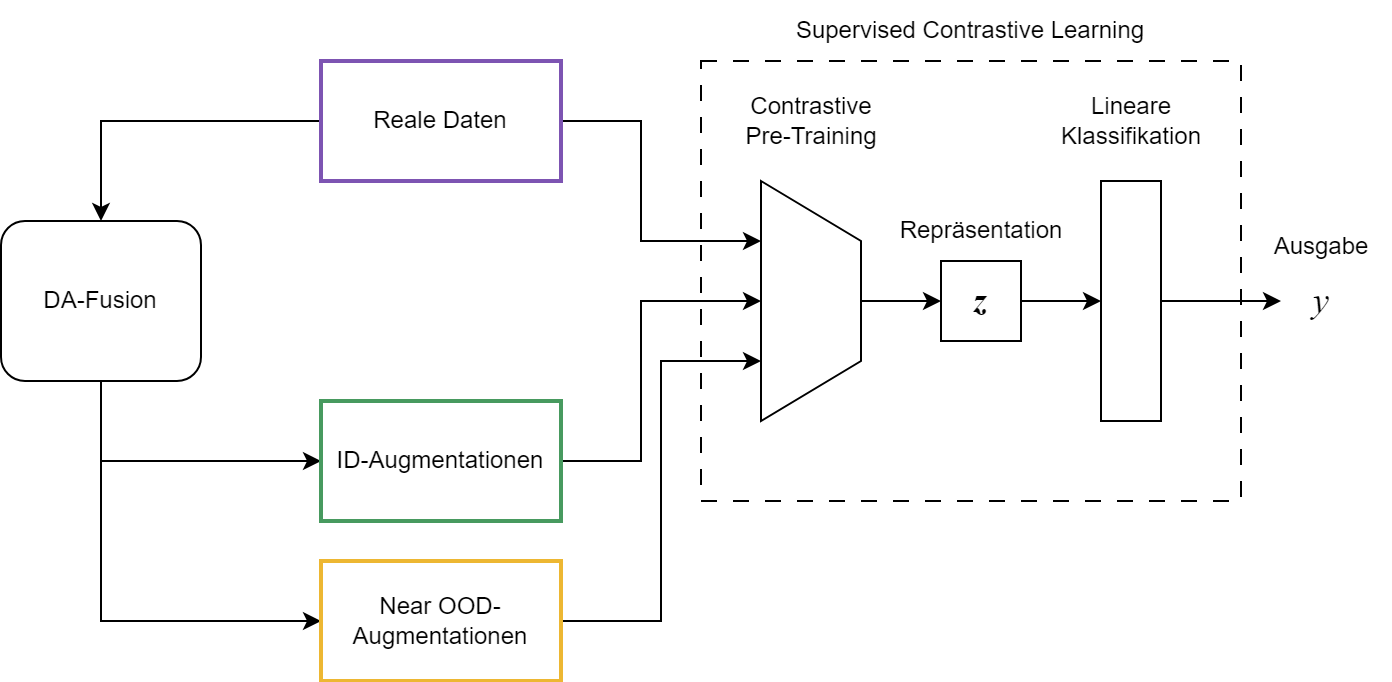
\includegraphics[width=\textwidth]{figure_flowchart.png}
	\caption{Übersicht des Versuchsaufbaus für die Generierung der synthetischen Daten mit DA-Fusion und die Trainings- und Testdurchläufe mit Supervised Contrastive Learning.}
	\label{fig:experiment-setup}
\end{figure}

\subsection{Synthetische Datengenerierung} \label{subsec:da-fusion-setup}

% ID- & Near OOD-Augmentationen
Es wurden mit DA-Fusion zwei unterschiedliche Sätze von Augmentationen generiert: die In-Distribution-Augmentationen und die Near Out-of-Distribution-Augmentationen.

% Textual Inversion Finetuning:
	% model="CompVis/stable-diffusion-v1-4"
	% initializer_token="motor"
	% num_vectors=16
	% resolution=512
	% examples_per_class=32
	% train_batch_size=16
	% lr=5.0e-04
	% lr_scheduler="constant_with_warmup"
	% lr_warmup_steps=150
	% mixed_precision=fp16
	% max_train_steps=1000
Für beide Sätze wurde als vortrainiertes Modell \lstinline{CompVis/stable-diffusion-v1-4}\footnote{\url{https://huggingface.co/CompVis/stable-diffusion-v1-4}} ausgewählt. Es wurden 32 Beispielbilder pro Klasse für das Training ausgewählt. Die Klassen wurden alle mit dem Token \lstinline{<motor>} initialisiert. Dabei wurden über das Argument \lstinline{num_vectors} 16 Textual Inversion Vektoren pro Text-Embedding verwendet. Das Finetuning erfolgte mit einer Bildgröße von 512x512 Pixeln,einer Batch Size von 16, einer Lernrate von 0.0005 und einer konstanten Lernrate mit Warmup über 150 Schritte. Es wurde Mixed Precision mit FP16 verwendet und das Training wurde nach 1000 Schritten beendet. Die erlernten Text-Embeddings wurden für beide Sätze verwendet, um die Augmentationen zu generieren.

% Generierung:
	% aug="real-guidance"
	% guidance_scale=15
	% prompt="a photo of a {}"
	% strength=0.2/0.5
	% examples_per_class=16
	% num_synthetic=4
Die Generierung erfolgte mit einer Guidance Scale von 15. Es wurden 16 Beispiele pro Klasse zur Augmentation herangezogen und für jedes Beispiel vier synthetische Bilder generiert. Die Segmentierungsmasken wurden verwendet, um die Augmentation nur auf den Bereich des Objekts zu begrenzen. Die ID- und Near OOD-Augmentationen unterscheiden sich nur durch den \lstinline{strength}-Parameter, wobei für die ID-Augmentationen ein Wert von \textbf{0.2} und für die Near OOD-Augmentationen ein Wert von \textbf{0.5} verwendet wurde.

\subsection{Trainings- und Testdurchläufe} \label{subsec:supcon-setup}

% Drei Versuche; jeweils Contrastive Pre-Training & Lineare Klassifikation
Die Trainings- und Testdurchläufe mit Supervised Contrastive Learning sind in drei Versuchsreihen unterteilt. In jedem Versuch wird zunächst das Pre-Training der latenten Repräsentationen durchgeführt, gefolgt von der linearen Klassifikation der Repräsentationen. Die Versuchsreihen unterscheiden sich in der Verwendung der synthetischen Augmentationen:

\begin{itemize} %[font=\bfseries]
	\item \emph{Versuch 1}: Nur reale Daten werden verwendet, sowohl für das Pre-Training als auch für das Training des Klassifikators.
	\item \emph{Versuch 2}: Neben den realen Daten werden auch ID-Augmentationen verwendet, sowohl für das Pre-Training als auch für das Training des Klassifikators.
	\item \emph{Versuch 3}: Wie Versuch 2, aber im Pre-Training werden zusätzlich Near OOD-\\Augmentationen verwendet, wie in \autoref{subsec:da-fusion-supcon} beschrieben.
\end{itemize}

% Hyperparameter
Für das Pre-Training wurde eine Batch Size von 16, eine Lernrate von 0.001 mit Kosinus-Annealing und einer Dauer von 110 Epochen verwendet. Die Bilddaten wurden im Rahmen der herkömmlichen Augmentation, welche die zwei Ansichten eines Beispiels erzeugt, auf eine Größe von 224x224 Pixeln zugeschnitten und normalisiert.

Bei der linearen Klassifikation sind die Hyperparameter identisch, jedoch mit einer Dauer von nur 25 Epochen. Nach jeder Trainingsepoche werden die Modelle für eine Validierungsepoche auf den (echten) Testdaten evaluiert.

\subsection{Evaluationsmethoden und Metriken} \label{subsec:evaluation}

% Accuracy, ID- und OOD-Confidence des SCL Klassifikators
Die drei Versuchsreihen werden ausgewertet, indem folgende Metriken beim Test der linearen Klassifikation auf den Testdaten gemessen werden:

\begin{itemize}
	\item \emph{Top-1 Accuracy}: Der Anteil der korrekt klassifizierten Bilder. Top-1 bedeutet, dass das Modell die Klasse mit der höchsten Wahrscheinlichkeit als Vorhersage ausgibt.
	\item \emph{ID-Confidence}: Die durchschnittliche Konfidenz des Klassifikators auf den ID-Daten. Die Konfidenz ist die Wahrscheinlichkeit, die der Klassifikator für die Vorhersage der korrekten Klasse ausgibt.
	\item \emph{OOD-Confidence}: Die durchschnittliche Konfidenz des Klassifikators auf den OOD-Daten.
\end{itemize}

% Menschliche Evaluierung der Augmentationen selbst
Vor der Auswertung der Versuchsreihen wurde eine menschliche Evaluierung der synthetischen Daten durchgeführt. Dabei wurde bewertet, ob die Objekte in den Bildern in ihrer Form und Struktur unverändert bleiben, während die Farben und Texturen variieren können und sollen. Bei den OOD-Augmentationen wurde darauf geachtet, dass die Objekte so stark verändert werden, dass eine Klassifizierung in die ursprüngliche Objektklasse als fehlerhaft angesehen wird. Gleichzeitig sollten die OOD-Beispiele noch genug Ähnlichkeit aufweisen, um herausfordernde negative Beispiele zu sein.